% !TEX TS-program = pdfLaTeX+MakeIndex+BibTeX
% !TEX encoding = UTF-8 Unicode

\PassOptionsToPackage{unicode}{hyperref}
\PassOptionsToPackage{naturalnames}{hyperref}

\documentclass[tg]{mdtufsm}

\usepackage[T1]{fontenc}
\usepackage{fix-cm}
\usepackage{microtype} % Nicer text flowing & typography
\usepackage{times, color}
\usepackage[utf8]{inputenc}
\usepackage{graphicx}
\usepackage{amsmath,latexsym,amssymb}
%\usepackage[hidelinks]{hyperref}
\usepackage[hidelinks,
            bookmarksopen=true,linktoc=none,colorlinks=true,
            linkcolor=black,citecolor=black,filecolor=magenta,urlcolor=blue,
            pdftitle={Desenvolvimento e Reutilização de Testes Automatizados em Aplicações Web},
            pdfauthor={Lucas Antunes Amaral},
            pdfsubject={Trabalho de Graduação},
            pdfkeywords={Qualidade de Software, Testes automatizados de Software, Linguagens de Programação, Selenium HQ, Cucumber, Informática, UFSM}
            ]{hyperref}
%\usepackage[brazilian]{babel}

%\usepackage{fontspec}
%\setmainfont{Linux Libertine G}

%%% PAGE DIMENSIONS
\usepackage[inner=30mm,outer=20mm,top=30mm,bottom=20mm]{geometry}
%\usepackage{epstopdf}
\usepackage{graphicx}
\usepackage{pdfpages}
% \geometry{margin=2in} % for example, change the margins to 2 inches all round
% \geometry{landscape} % set up the page for landscape

% \usepackage[parfill]{parskip} % Activate to begin paragraphs with an empty line rather than an indent

%%% PACKAGES
%\usepackage{amsfonts}
%\usepackage{color}
%\usepackage{booktabs} % for much better looking tables
%\usepackage{array} % for better arrays (eg matrices) in maths
%\usepackage{paralist} % very flexible & customisable lists (eg. enumerate/itemize, etc.)
\usepackage{siunitx}
%\usepackage{verbatim} % adds environment for commenting out blocks of text & for better verbatim
\usepackage{listings}
\usepackage{subcaption}
\captionsetup{compatibility=false}
%\usepackage{microtype}
%\usepackage[numbers]{natbib}
%\usepackage{subfig} % make it possible to include more than one captioned figure/table in a single float
% These packages are all incorporated in the memoir class to one degree or another...

\lstdefinelanguage{Java}{
  keywords={public, private, new, true, boolean, false, catch, void, return, null, for, switch, var, if, in, while, else, case, break, class,
  	Funcionalidade, Contexto, Dado, Quando, E, Entao, Cenario, Delineacao, Exemplos},
  keywordstyle=\color[rgb]{0.2,0.4,0.55}\bfseries,
  ndkeywords={export, throw, implements, import, this,
    @Before, @Test, @After, @Dado, @Quando, @E, @Entao, @Documented, @Retention, @Target, @Teste, @aceitacao, @rejeicao, codigoDis, nomeNovaDisciplina, relevancia, siglaInst, msgErro},
  %ndkeywords={Add, Num},
  ndkeywordstyle=\color[RGB]{218,202,66}\bfseries,
  %identifierstyle=\color{black},
  sensitive=true,
  comment=[l]{//},
  morecomment=[s]{/*}{*/},
  commentstyle=\color{purple}\ttfamily,
 % stringstyle=\color[rgb]{0.0,0.4,0.65}\ttfamily,
  stringstyle=\color[RGB]{34,128,24}\ttfamily,
  %morestring=[b]',
  morestring=[b]"
}

\lstset{
	language=Java,
	basicstyle=\tiny,
	commentstyle=\color[rgb]{0,0.2,0}\normalfont,
	frame=single,
	%texcl=true,
	numbers=left,
	showstringspaces=false,
}

\lstset{
	basicstyle=\scriptsize\ttfamily,
	tabsize=2,
	frame=single,
	breaklines=true,
	breakatwhitespace=true,
	xleftmargin=0cm,
	xrightmargin=0cm,
	literate=
		{á}{{\'a}}1 {é}{{\'e}}1 {í}{{\'i}}1 {ó}{{\'o}}1 {ú}{{\'u}}1
		{Á}{{\'A}}1 {É}{{\'E}}1 {Í}{{\'I}}1 {Ó}{{\'O}}1 {Ú}{{\'U}}1
		{à}{{\`a}}1 {è}{{\`e}}1 {ì}{{\`i}}1 {ò}{{\`o}}1 {ù}{{\`u}}1
		{À}{{\`A}}1 {È}{{\'E}}1 {Ì}{{\`I}}1 {Ò}{{\`O}}1 {Ù}{{\`U}}1
		{ä}{{\"a}}1 {ë}{{\"e}}1 {ï}{{\"i}}1 {ö}{{\"o}}1 {ü}{{\"u}}1
		{Ä}{{\"A}}1 {Ë}{{\"E}}1 {Ï}{{\"I}}1 {Ö}{{\"O}}1 {Ü}{{\"U}}1
		{â}{{\^a}}1 {ê}{{\^e}}1 {î}{{\^i}}1 {ô}{{\^o}}1 {û}{{\^u}}1
		{Â}{{\^A}}1 {Ê}{{\^E}}1 {Î}{{\^I}}1 {Ô}{{\^O}}1 {Û}{{\^U}}1
		{ã}{{\~a}}1 {Ã}{{\~A}}1 {õ}{{\~o}}1 {Õ}{{\~O}}1
		{ç}{{\c c}}1 {Ç}{{\c C}}1,
	texcl=true,
	%numbers=left,
	showstringspaces=false,
	commentstyle=\normalfont
}

% For Computer Modern:
%\def\Cpp{{C\nolinebreak[4]\hspace{-.05em}\raisebox{.4ex}{\tiny\bf ++}}}
% For Linux Libertine G
\def\Cpp{{C\nolinebreak[4]\raisebox{.20ex}{\small\bf++}}}

%\newcommand{\todo}[1]{\textsf{\color{red}#1}}
\newcommand{\todo}[1]{}
\graphicspath{{./images/}}

%%=============================================================================
%% Trampa para corrigir o bug do hyperref que redefine o caption das figuras e das
%% tabelas, não colocando o nome ``Figura'' antes do número do mesmo na lista
%%=============================================================================

\makeatletter

\long\def\@caption#1[#2]#3{%
  \expandafter\ifx\csname if@capstart\expandafter\endcsname
                  \csname iftrue\endcsname
    \global\let\@currentHref\hc@currentHref
  \else
    \hyper@makecurrent{\@captype}%
  \fi
  \@ifundefined{NR@gettitle}{%
    \def\@currentlabelname{#2}%
  }{%
    \NR@gettitle{#2}%
  }%
  \par\addcontentsline{\csname ext@#1\endcsname}{#1}{%
    \protect\numberline{\csname fnum@#1\endcsname ~-- }{\ignorespaces #2}%
  }%
  \begingroup
    \@parboxrestore
    \if@minipage
      \@setminipage
    \fi
    \normalsize
    \expandafter\ifx\csname if@capstart\expandafter\endcsname
                    \csname iftrue\endcsname
      \global\@capstartfalse
      \@makecaption{\csname fnum@#1\endcsname}{\ignorespaces#3}%
    \else
      \@makecaption{\csname fnum@#1\endcsname}{%
        \ignorespaces
        \ifHy@nesting
          \expandafter\hyper@@anchor\expandafter{\@currentHref}{#3}%
        \else
          \Hy@raisedlink{%
            \expandafter\hyper@@anchor\expandafter{%
              \@currentHref
            }{\relax}%
          }%
          #3%
        \fi
      }%
    \fi
    \par
  \endgroup
}

\makeatother

%%% END Article customizations

\title{Desenvolvimento e Reutilização de Testes Automatizados em Aplicações Web}
\author{Amaral}{Lucas Antunes}
\course{Curso de Ciência da Computação}
\altcourse{Curso de Ciência da Computação}
\institute{Centro de Tecnologia}
\degree{Bacharel em Ciência da Computação}

\trabalhoNumero{}
\advisor[Profª.]{Drª.}{Charão}{Andrea Schwertner}
\orientadoratrue

\committee[Profª. Dr.]{Bernardi}{Giliane}{UFSM}
\committee[MSc.]{Pereira}{Adriano}{UFSM}

\date{4}{Dezembro}{2015}

\keyword{Qualidade de Software}
\keyword{Testes automatizados de Software}
\keyword{Linguagens de Programação}
\keyword{Selenium HQ}
\keyword{Cucumber}

%\date{} % Activate to display a given date or no date (if empty), otherwise the current date is printed

\begin{document}
\maketitle
\makeapprove
%\includepdf[pages={-}]{folha_de_aprovacao.pdf}

\chapter*{Agradecimentos}
Agradeço e dedico este trabalho, em primeiro lugar, aos meus filhos Anna Clara e Bernardo, por serem minha inspiração e por tornarem importante e válido cada dia ao longo desse processo, estimulando-me sempre com seus sorrisos e carinhos. Agradeço a minha esposa, Ariane Mattezdolf, pelo companheirismo em todos os momentos. 

Agradeço aos meus pais Dina Antunes e Éder Amaral, pelo apoio incondicional e por me tornarem a pessoa que hoje sou. Também a minha irmã, amiga e professora, Larissa Amaral.

Em especial, agradeço a minha professora e orientadora Andrea Charão, por sua paciência e dedicação ao conduzir-me durante a elaboração e desenvolvimento deste trabalho. Aos membros de minha banca, professora Giliane Bernardi e Adriano Pereira, pelas sugestões e comentários construtivos feitos na sessão prévia de apresentação do trabalho em questão.  

Também agradeço aos meus amigos e demais familiares que, de uma forma ou outra, fizeram parte desta trajetória, dividindo momentos de descontração e amizade comigo.
\begin{abstract}
A constante busca pela qualidade de uma solução em forma de software, fez com que empresas do ramo de desenvolvimento aderissem a realização de testes automatizados em seus sistemas. A partir deste cenário,
surgiram inúmeras ferramentas e \emph{frameworks} para suprir esta demanda, que se propõem  a ampliar a otimização de tempo e eficácia das aplicações implementadas, visando uma garantia maior na qualidade das mesmas. Contudo, é sabido que criar um novo teste para cada nova funcionalidade ou demanda do sistema, torna-se muito custoso, sendo necessário um grande desprendimento de recursos humanos. Assim, este trabalho apresenta abordagens reutilizáveis de teste que objetivam trazer praticidade e facilidade na confecção de novos testes, utilizando para isso métodos de classes genéricas de testes confeccionados no mesmo, especificamente voltados para sistemas web desenvolvidos na linguagem de programação Java.
\end{abstract}

\begin{englishabstract}
{Development and Re-use Automated Test Web Applications}
{Undergraduate Program in Computer Science}
{Software Quality, Automated Test Software, Programming Languages, Selenium HQ, Cucumber}
{December}
{nd}
The ongoing need for a reliable software solution, compelled development companies to perform automated testing of their systems. From that context, several tools and frameworks emerged to address this need, aiming to improve time optimization and effectiveness of the implemented applications, increasing the assurance of their quality. However, developing a new test for every new functionality or system need is known to be costly and highgly demanding of human resources. Therefore, this work presents reusable testing approaches to allow convenient and easy development of new tests, making use of generic methods that are specifically focused on web systems developed with Java programming language.
\end{englishabstract}

\tableofcontents
\listoffigures
\listoftables
%\listofappendix

\setlength{\baselineskip}{1.5\baselineskip}

%	\item[Período de execução:] Setembro de 2014 a Dezembro de 2014
%	\item[Unidades participantes:] ~\\ Curso de Ciência da Computação \\ Departamento de Eletrônica e Computação
%	\item[Área de conhecimento:] Ciência da Computação
%	\item[Linha de Pesquisa:] Computação Gráfica, Linguagens de Programação, Programação Paralela
%	\item[Tipo de projeto:] Trabalho de Conclusão de Curso

\chapter{Introdução}

Dada a atual conjectura do mercado de desenvolvimento de software é fundamental, para
que uma aplicação se mantenha viva de forma competitiva, apresentar diferenciais ao seu público alvo. Desta maneira, a área de qualidade de software ganha cada vez mais espaço dentro das empresas de tecnologia da informação e, em especial, as ferramentas e
metodologias de teste de software ganham maior visibilidade. Além do aumento da produtividade e da diminuição do retrabalho, as empresas na área de tecnologia da informação buscam um melhor relacionamento com seus clientes por meio do melhor planejamento e gestão de suas atividades de desenvolvimento e da diminuição no número de defeitos nos produtos entregues \cite{jomori2004qualidade}.

Os testes de software podem ocorrer em todas as etapas do desenvolvimento e de diferentes formas, contudo,
sempre objetivam atender na totalidade os requisitos do sistema e, simultaneamente, amplificar a qualidade da solução
codificada. Apesar de, aparentemente, ser mais prático e rápido realizar um teste manual, a cada nova alteração em um módulo do sistema,
o teste tem que ser todo refeito e a tendência que novos erros sejam gerados, até mesmo em funcionalidades já testadas, é enorme,
problema este que não ocorre quando a abordagem escolhida é a automatização dos testes. 

Os testes automatizados angariam cada vez mais adeptos ao longo dos últimos anos. Tal fato se deve principalmente à grande redução de custo observada a médio e longo prazos com o uso desta prática \cite{de2007utilizaccao}. Em contrapartida, os testes automatizados demandam um grande custo inicial em sua codificação e, com isso, aumentam o
envolvimento da equipe de qualidade. Pensando nesse problema, podemos buscar formas alternativas para que se possa usufruir de todas estas virtudes dos testes automatizados e, ao mesmo tempo, utilizar de forma eficiente os recursos disponíveis em uma instituição.

\section{Objetivos}

\subsection{Objetivo geral}

Este trabalho tem como objetivo principal apresentar um conjunto de classes de teste e testes que possam ser reutilizados em novas funcionalidades de uma aplicação ou em sistemas que sigam os mesmos padrões e comportamento dos softwares para os quais foram desenvolvidos visando agilizar o desenvolvimento dos testes.

\section{Justificativa}

A qualidade de software  é uma das variáveis essenciais para que um projeto de software tenha sucesso.
Sendo assim, torna-se cada vez mais necessária a inserção de testes automatizados em projetos web agregando, aos mesmos, uma maior confiabilidade e redução nos possíveis
erros que o sistema possa apresentar. Para que haja a possibilidade de aumentar a qualidade dos sistemas, sem que seja necessária uma maior
demanda de recursos humanos para a área de qualidade, podemos adotar práticas de reuso de códigos de testes, visando
maximizar a produtividade e eficiência, além de, simultaneamente, obter um produto final com uma garantia de qualidade
superior.

\section{Abordagem metodológica}
A seguir será descrita a sequência de passos que foram realizados neste trabalho
objetivando agilizar a confecção de testes de software em um projeto.

\subsection{Desenvolvimento de solução para testes unitários}
Como primeiro passo deste trabalho, desenvolveu-se uma solução composta por anotações na linguagem Java e a execução dos testes através da ferramenta Selenium WebDriver.
Essa solução, permite descrever testes unitários apenas inserindo anotações aos métodos de uma classe Java.

\subsection{Desenvolvimento de solução para testes funcionais com Cucumber}
A fim de possibilitar a confecção de testes funcionais, criou-se uma nova abordagem composta pela utilização da linguagem Cucumber e o \emph{framework} Selenium WebDriver.
Cucumber possibilitou descrever testes para funcionalidades do sistema, através de cenários em uma linguagem que se aproxima da linguagem natural.

\subsection{Desenvolvimento de solução para testes funcionais utilizando Selenium}
Como meio de apresentar uma solução que permitisse testes funcionais com elementos mais complexos, como testes condicionais e manipulação de objetos Java, desenvolveu-se
uma terceira abordagem neste trabalho, onde a mesma seguia os moldes da abordagem anterior, diferindo-se apenas na forma como os testes funcionais eram descritos. Ao invés de
escreve-los por meio da linguagem Cucumber, os mesmo foram descritos por métodos e classes Java, utilizando para isso recursos disponibilizados pela ferramenta Selenium.

\subsection{Comparações entre as soluções}
O ultimo passo deste trabalho, consistiu em apresentar comparações entre as soluções propostas, apresentando virtudes e limitações de cada uma. Também demonstrou-se
vantagens na utilização das abordagens funcionais deste trabalho ao detrimento de desenvolver um teste, utilizando apenas as ferramentas para testes de sistemas web disponíveis.

\chapter{Fundamentos e revisão de literatura}

Neste capítulo, serão apresentados conceitos relativos aos conteúdos abordados neste trabalho, descrevendo qualidade de software, ferramentas de teste de software, assim como, o reuso de testes.

\section{Qualidade de software}

A qualidade de software é uma subárea, oriunda da engenharia de software, que tem como foco central apresentar metodologias,
procedimentos e métricas que garantam a qualidade no processo de desenvolvimento de um sistema. Apesar de ocorrer no processo, a qualidade de software
objetiva obter qualidade no produto final e, com isso, conseguir contemplar na totalidade os requisitos tratados com o cliente ao longo do processo.
\citeauthor{de2006introduccao} (\citeyear{de2006introduccao}) afirmam que a qualidade de software está diretamente relacionada a um gerenciamento
rigoroso de requisitos, uma gerência efetiva de projetos e em um processo de desenvolvimento bem definido gerenciado e em melhoria contínua. Afirmam também,
que atividades de verificação e uso de métricas para controle de projetos e processo também estão inseridas nesse contexto, contribuindo para tomadas de
decisão e para antecipação de problemas.

Mas como medir a qualidade de um sistema em questão? Para responder este questionamento, \citeauthor{garvin1987competing} (\citeyear{garvin1987competing}) propõe o conceito que ele chama de
oito dimensões que seriam, em ordem, qualidade do desempenho, qualidade dos recursos, confiabilidade, conformidade, durabilidade, facilidade de manutenção,
estética e percepção. Segundo \citeauthor{garvin1987competing}, atendendo a estes oito critérios, o sistema apresentará qualidade.
\citeauthor{pressman2011engenharia} (\citeyear{pressman2011engenharia}) complementa a definição de Garvin, mesclando-a com a norma ISO 9126 e, aponta os fatores
críticos para o sucesso neste caso, como sendo: Intuição, Eficiência, Robustez e Riqueza.

\subsection{Qualidade do processo}
A qualidade de software é largamente determinada pela qualidade dos processos utilizados para o desenvolvimento. Deste modo, a melhoria
da qualidade de software é obtida pela melhoria da qualidade dos processos \cite{koscianski2007qualidade}.

\subsection{Qualidade do produto}
Existe uma relação direta entre qualidade de produto e qualidade do processo, pois, para obtenção da qualidade do produto final,
faz-se necessário adquirir, primeiramente, qualidade nos processos que compõem o desenvolvimento do mesmo.
Avaliar a qualidade de um produto de software é verificar, através de técnicas e atividades operacionais, o quanto os requisitos são atendidos. Tais requisitos,
de uma maneira geral, são a expressão das necessidades, explicitados em termos quantitativos ou qualitativos e tem por objetivo definir as características de
um software, a fim de permitir o exame de seu atendimento \cite{koscianski2007qualidade}.

\section{Testes de software}
É a atividade responsável por apresentar os erros existentes em um determinado programa. Por isso, pode ser vista como uma atividade destrutível, pois visa expor os defeitos para depois corrigir os mesmos e, de preferência, em
um estágio inicial. Quanto mais tarde um defeito for identificado, mais caro fica para corrigi-lo e, mais, os custos de descobrir e corrigir o defeito no software aumentam exponencialmente na proporção em que o trabalho
evolui através das fases do projeto de desenvolvimento \cite{boehm1976quantitative}. O teste possibilita também validar se os requisitos inicias do sistema, alinhados pelos \emph{stakeholders}, estão contemplados em sua plenitude.

Apesar de não ser possível, através de testes, provar que um programa está correto, os testes, se conduzidos sistemática e criteriosamente, contribuem para
aumentar a confiança de que o software desempenha as funções especificadas e evidenciar algumas características mínimas do ponto de vista da qualidade do produto \cite{maldonado2004introduccao}. Sendo assim,
faz-se essencial o mapeamento de um processo de testes para que se possa criar garantias e métricas que reduzam os erros, maximizando a qualidade. \citeauthor{crespo2004metodologia} (\citeyear{crespo2004metodologia}) descrevem o processo de
teste como sendo a composição de quatro macro etapas: planejamento, projeto, execução e acompanhamento dos testes de unidade.

\subsection{Caso de teste}
O propósito do caso de teste é definir uma unidade de teste que será executada pelo testador, seja manual ou automaticamente \cite{rios2006teste}. Um caso de teste é constituído visando descrever passos sequenciais necessários para validação de um artefato de teste. O caso de teste deve especificar a saída esperada e os resultados esperados do processamento \cite{myers2011art}.

\subsection{Tipos de teste}
Existem muitos tipos de teste, mas podemos destacar entre elas: teste de unidade, integração, sistema, aceitação e regressão. Serão descritos nas próximas subseções os tipos utilizados no desenvolvimento deste trabalho.

\subsubsection{Teste unitário}
O teste de unidade focaliza o esforço de verificação na menor unidade de projeto do software \cite{pressman2011engenharia}. Em uma aplicação orientada a objeto, o teste, neste caso, seria voltado ao método.

\subsubsection{Teste funcional}
Baseando-se numa descrição \emph{black-box} da funcionalidade do software, o teste funcional é capaz de checar se o software está de acordo com sua especificação independentemente da sua implementação \cite{fantinato2005autotest}.
 
\subsection{Estratégias de testes}
A estratégia de testes se caracteriza pela definição da abordagem geral a ser aplicada nos testes, descrevendo como o software será testado, identificando os níveis de testes que serão aplicados, os métodos,
técnicas e ferramentas a serem utilizada \cite{rios2006teste}. Deve-se também escolher na etapa de estratégia os tipos de testes que deverão ser realizados, assim como os estágios de teste escolhidos. Uma estratégia de teste de software deve acomodar testes de baixo nível, necessários para verificar se um pequeno segmento de código fonte foi implementado corretamente, bem com testes de alto nível, que validam as funções principais do sistema de acordo com os requisitos do cliente \cite{pressman2011engenharia}.

Tradicionalmente, entre desenvolvedores de teste, utiliza-se uma estratégia onde temos um equilíbrio entre testar o sistema após pronto e testar somente antes de desenvolver o sistema. Esta estratégia assume uma visão incremental do teste, começando com o teste de unidades individuais de programa, passando para os testes destinados a facilitar a integração de unidades e culminando com testes que usam o sistema concluído \cite{pressman2011engenharia}.

\subsection{Testes de sistemas web}
O teste de aplicações Web se reveste de características peculiares, uma vez que se tratam, em geral, de aplicações colocadas na Internet e cujo acesso, em teoria,
é aberto a qualquer usuário \cite{rios2006teste}.  De forma geral, as aplicações web diferem-se dos sistemas \emph{Desktop} pelos cuidados necessários com questões como a
possibilidade de utilização de sistemas operacionais e navegadores distintos, segurança e conectividade. Além disso, a relevância econômica das aplicações Web aumenta a
importância de controlar e de melhorar a sua qualidade \cite{fidelis2004fireweb}.


\section{Ferramentas para teste de software}
Existem muitas ferramentas desenvolvidas para realização de testes de software web. Neste trabalho serão descritas três(3) dentre elas, que serão as ferramentas utilizadas no desenvolvimento dos testes estudados.

\subsection{Selenium HQ}
É um \emph{framework} open source utilizado para automatização de testes funcionais em aplicações web \cite{chiavegatto1desenvolvimento}. Segundo \citeauthor{pereiraestudoselenium} (\citeyear{pereiraestudoselenium}) se trata
de uma ferramenta de fácil uso e eficiente para desenvolver casos de teste, permitindo os testes de aceitação ou funcional, regressão e de desempenho.
Selenium trabalha como um plugin do navegador Firefox, o mesmo traz muita praticidade, pois permite que se possa capturar cliques e valores digitados, transformando-os em um caso de teste. Ele é composto por
quatro ferramentas: Selenium IDE, Selenium Grid, Selenium RC e Selenium WebDrive.

A utilização de comandos no Selenium consiste em digitar o comando seguido de dois parâmetros tal como, por exemplo, \texttt{verifyText //div//a[2] Login}. Dependendo  do comando os parâmetros poderão ser opcionais, pois, alguns comandos não necessitam de parâmetros para serem executados \cite{sixpenceautomatizaccao}.

Selenium foi escolhida como umas das ferramentas no desenvolvimento deste projeto pelo fato de ser um \emph{framework open source} que possui um vasto leque de ferramentas para testes de sistemas web. Outro fator
importante para sua escolha é a possibilidade de interação do Selenium HQ com o Cucumber. Ela se destaca entre as demais ferramentas gratuitas pelo fato de ser a mais completa, permitindo integração com
várias linguagens, outros \emph{frameworks}, além de suportar inúmeros navegadores e sistemas operacionais \cite{pereiraestudoselenium}.

\subsection{Cucumber}
Cucumber é uma ferramenta de desenvolvimento de testes, voltada para sistemas web, que adota uma linguagem de alto nível bem próxima a uma linguagem natural e tem suas origens fixadas sobre a metodologia BDD (\emph{Behavior Driven Development}). Cucumber
é escrita em linguagem Ruby, mas pode ser utilizada para executar especificações de aplicações escritas em qualquer linguagem \cite{nunescucumber}.

A escolha dessa ferramenta baseou-se na fácil transcrição dos requisitos do sistema para a linguagem em questão, tornando possível conferir se os requisitos estão contemplados pelas funções e métodos descritos no sistema web.
\citeauthor{lopescucumbervalor} (\citeyear{lopescucumbervalor}) compara Cucumber com o software Capybara\footnote{Capybara é uma biblioteca escrita na linguagem de programação Ruby que torna fácil simular como um usuário interage com sua aplicação. http://jnicklas.github.io/capybara/} e afirma que o primeiro apresenta um código mais legível e amigável. Uma observação é que o código com Capybara faz
referência para vários detalhes de implementação, enquanto o código do Cucumber reserva isso apenas para os \emph{Steps} e não para o arquivo de \texttt{feature} \cite{lopescucumbervalor}.

A ferramenta funciona, basicamente, através da leitura de arquivos com a extensão \texttt{feature}, os quais descrevem em linguagem natural uma funcionalidade e casos de teste, conhecidos como cenários.
Como os testes estão escritos em uma linguagem natural e não de programação, Cucumber precisa pesquisar pelo código associado aos passos que formam o cenário em arquivos auxiliares \cite{scmitzcucumberreview}. Cucumber
executa seus arquivos \texttt{.feature} e esses arquivos contêm especificações executáveis escritos em uma linguagem chamada Gherkin \cite{cucumberwiki}, que possui um layout bem definido. Inicia pela descrição de uma funcionalidade
que, por sua vez, possui cenários; onde, um cenário é descrito da seguinte forma: \texttt{Dado} alguma condição \texttt{Quando} outra condição \texttt{E} terceira condição \texttt{Então} faça algo, conforme ilustra a figura \ref{fig:codigo_cucumber}.

\begin{figure}[!htb]
	\centering
	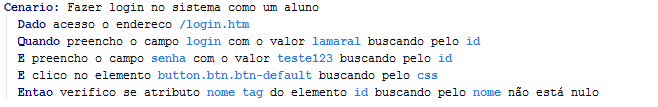
\includegraphics[width=1.1
	\textwidth]{codigo_cucumber}
	\caption{Um exemplo de código cucumber.}
	\label{fig:codigo_cucumber}
\end{figure}

\subsection{JUnit}
JUnit é uma ferramenta de apoio ao teste unitário, a qual auxilia desenvolvedores na automação dos testes e verificação dos resultados \cite{biasi2006geraccao}. A escolha desta ferramenta, como parte integrante da solução desenvolvida, deveu-se ao fato da mesma ser voltada para sistemas desenvolvidos na linguagem de programação Java, além de ser altamente versátil, possibilitando, assim, integração em um único código da mesma com os demais \emph{frameworks} que serão utilizados (Selenium e Cucumber).

Justifica-se a sua utilização neste trabalho por tratar-se de uma API (\emph{Application Programming Interface}), que viabiliza a comparação de um valor obtido em algum teste com o valor esperado pelo mesmo. Desta forma, pode-se validar e verificar se
a funcionalidade de um sistema está trabalhando adequadamente.

\section{Reuso de testes}

Visando melhor aproveitar os recursos existentes em uma instituição e, ainda assim, apresentar garantias na qualidade do produto/serviço entregues aos clientes, desenvolvedores do mundo todo começaram a apresentar
teses e modelos que buscam criar testes genéricos e padronizados. Um padrão é um pedaço de informação instrutiva e nomeada, que captura a estrutura essencial
e \emph{"insights"}, de uma família bem sucedida de soluções aprovadas, para um determinado problema, o qual surge em um determinado contexto \cite{cagnin2004reuso}.

\citeauthor{guizzardi2000desenvolvimento} diz que, por razões históricas, a área de desenvolvimento de software não atingiu a maturidade que outras áreas da engenharia atingiram. Complementa afirmando que, apesar disso, é inegável que algum avanço tenha sido alcançado, pois a forma de realização dessa atividade evoluiu de uma atividade realizada de forma quase artesanal, para um processo de
desenvolvimento bem estruturado e que, nos melhores casos, contempla inclusive atividades de gerência e avaliação da qualidade \cite{guizzardi2000desenvolvimento}.
Com isso, a reutilização dos testes já codificados se mostra uma importante prática no desenvolvimento e que ainda apresenta muitas incógnitas e possibilidades para as equipes de TI,
principalmente na geração de casos de testes que possam ser reutilizados em situações que apresentem um padrão parecido com os casos já conhecidos.

Como solução em forma de reutilização de teste, \cite{cagnin2004reuso} apresentam uma abordagem composta por: a) uma estratégia, que define e associa requisitos de teste a padrões de linguagens de padrões  de análise; b) diretrizes, que apoiam o engenheiro de software na decisão de quais requisitos de teste disponíveis devem ser reusados e instanciados para casos de teste concretos. A estratégia que define os requisitos de teste da abordagem proposta foi aplicada aos padrões de uma
linguagem de padrões de análise, utilizados na reengenharia de um sistema legado de biblioteca. Já \cite{karinsalo2004software} sugerem um modelo de processo de desenvolvimento de teste que leva técnicas de reutilização de software e atividades em conta, revela ainda que, a fim de produzir material de teste reutilizável, as entidades de software têm de ser expressa em termos de recursos, em que os materiais de ensaio estão anexados.

Segundo \cite{patel2014test}, Tata Consultancy Services (TCS)  é uma empresa provedora de serviços em TI (ITSP) que desenvolveu um repositório de casos de teste reutilizáveis com o objetivo de reduzir o custo dos testes em projetos de Implementação de software empresarial (ESI).\cite{patel2014test} trás um estudo do programa de reutilização para analisar o seu impacto. Um conjunto de métricas foram definidos e os dados pertinentes foram obtidas a partir de usuários do repositório.

\cite{crespo2004metodologia} apresentam uma metodologia para implantação ou melhoria do processo de teste em empresas desenvolvedoras de software, com o objetivo de viabilizar a utilização das práticas de teste pelas empresas. Apesar de não tratar-se de uma solução que contenha reutilização de software este trabalho tem relação direta com o trabalho desenvolvido, pois a reutilização nada mais visa que melhorias no processo de desenvolvimento dos testes de software.

\chapter{Desenvolvimento}

A seguir serão descritas as atividades desenvolvidas a fim de alcançar os objetivos propostos por este trabalho. Será apresentado o escopo do projeto, assim como trechos dos códigos desenvolvidos e estrutura das soluções encontradas ao longo do desenvolvimento do projeto.

\section{Delimitação de escopo}

Como escopo, foram delimitados alguns pré-requisitos necessários para utilização da solução proposta neste trabalho, onde o sistema deve ser um software web desenvolvido na linguagem de programação Java,
podendo apresentar também funções Ajax e Javascript.

\section{Solução para testes unitários com anotações e Selenium}
Em um primeiro momento, com objetivo de automatizar os testes de uma aplicação a fim de reduzir o esforço na confecção e codificação de novos testes para as equipes de desenvolvimento e testes de uma organização,
escolheu-se desenvolver uma solução baseada em três etapas que são descritas conforme imagem \ref{fig:solucao1}.

\begin{figure}[!htb]
	\centering
	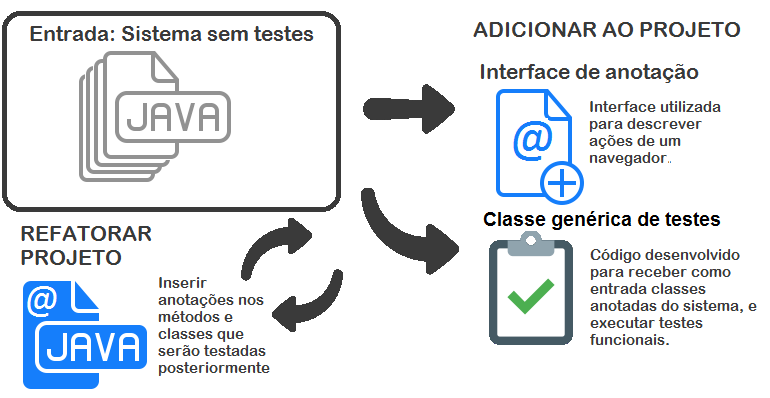
\includegraphics[width=0.8\textwidth]{solucao1}
	\caption{Estrutura da solução.}
	\label{fig:solucao1}
\end{figure}

Temos como ponto de partida um sistema onde se possui pouco ou nenhum teste codificado. Para o mesmo descrevemos  três fases no desenvolvimento de uma solução, em forma de testes para o sistema,
que seriam: criar uma classe de testes genérica, responsável por realizar os testes necessários na aplicação; descrever uma interface de anotação, que representaria ações de elementos web (\emph{HTML}) que
seriam testados posteriormente e, por fim, inserir as anotações nos métodos e classes do sistema que devem ser testados nesta aplicação.

\subsection{Classe genérica de testes}
Por tratar-se de uma abordagem para sistemas web, optou-se pela utilização de dois \emph{frameworks} de testes, que possibilitam interações com elementos web, para confecção da classe responsável pela execução dos testes automatizados.
O primeiro é o Selenium. Através da utilização da classe \texttt{WebDrive}, contida em seu pacote, podemos descrever uma sequência de passos que são executados por um navegador, como cliques e inserção de dados em campos de um
formulário. Sendo assim, instanciando um objeto \texttt{WebDrive}, podemos iniciar um navegador e realizar uma série de instruções pré-determinadas para validar se a aplicação comporta-se de forma adequada.

Por fim, necessitamos validar se após realizar o preenchimento de formulários do software, o resultado obtido condiz com o resultado esperado. Neste momento é onde se faz necessária a adição de trechos de códigos Junit na classe de teste
desenvolvida, pois o mesmo disponibiliza em seu pacote um conjunto de métodos \emph{assert}, com os quais é possível comparar, por exemplo, se após salvar um formulário de cadastro, a mensagem de "cadastrado com sucesso" aparece na tela.
A imagem \ref{code:TestaFormularios.java} apresenta um trecho da classe confeccionada para realização dos testes.

\begin{figure}[!htb]
\begin{lstlisting}
@Test
public void testaFormularios() { //Método que executa os testes unitários
	for (Class classe : getCarregaClasses()) { //Interando nas classes do sistema
    		Teste testeClasse = TestePropriedades.teste(classe); //Busca valor @Teste classe
        if (testeClasse.fazerLogin()) { //Fazendo login no sistema
            LoginTeste.login(TestePropriedades.urlSistema, testeClasse.getSenha(), testeClasse.getLogin(), webDriver);
        }
        if (!testeClasse.getUrl().equals("")) { //Acessar URL
            webDriver.get(TestePropriedades.urlSistema + testeClasse.getUrl());
        }
        for(Method metodo: classe.getDeclaredMethods()) {
            Teste teste = TestePropriedades.teste(metodo);
            if (teste != null) {
                executaTeste(teste, true); //Executa testes para cada método
            }
        }
        executaTeste(testeClasse, false); //Executa testes da classe
        System.out.println("Formulário da classe " + classe.getName() + " testado!");
	}
}
\end{lstlisting}
    \caption{Classe genérica de teste desenvolvida}
	\label{code:TestaFormularios.java}
\end{figure}

A classe desenvolvida possui um método principal denominado \texttt{testaFormularios}, onde a ideia principal do mesmo seria buscar,
de forma recursiva, todas as classes do projeto anotadas pela interface que indica quais classes deverão ser testadas e para cada uma das mesmas cria-se elementos \texttt{webDrive} para executar as ações indicadas pela anotação.

\subsection{Interface de anotação}

Após finalizar o desenvolvimento da classe de testes genérica, passou a existir a necessidade de criar um mecanismo para informar, à classe de testes, quais seriam as validações necessárias. Para esta tarefa,
por tratar-se de projetos Java, resolveu-se criar uma interface de anotação que seria vinculada aos métodos e classes, onde seriam necessários executar os casos de teste posteriores. Desta forma, a classe \texttt{TestaFormulario.java},
responsável pela execução dos testes, varreria as classes do sistemas e, toda vez que encontrar uma classe anotada por essa interface, executaria um teste, onde, cada método que necessitaria de um teste possuiria, em sua anotação, o tipo do campo,
as ações que deveriam ser executas e o valor que deveria ser preenchido.

Deu-se o nome de \texttt{Teste.java} para a interface, e sua estrutura está ilustrada em \ref{code:Teste.java}.

\begin{figure}[!htt]
\begin{lstlisting}
@Documented
@Retention(RetentionPolicy.RUNTIME)
@Target({ElementType.TYPE, ElementType.METHOD})
public @interface Teste {
    String getUrl() default "";

    //findElement
    String getCampo() default ""; //campo html do formulário
    String getIdentificador() default "id"; //Informar se deve buscar um id, name, class ou css

    boolean isSelect() default false;

    String getValor() default ""; //utilizado como sendKeys e selectText
    boolean click() default false;
    boolean submit() default false;
    boolean limpar() default false;
	
		//Métodos referentes a classe
    String getTipoAssert() default "igual";
    String getCampoAssert() default "";
    String getIdentificadorAssert() default "id";
    String getValorEsperadoAssert() default "";
    String getAtributoCampoComparacaoAssert() default "texto";

    boolean fazerLogin() default false;
    String getLogin() default "colegiado";
    String getSenha()default "";
}
\end{lstlisting}
	\caption{Interface Teste}
	\label{code:Teste.java}
\end{figure}

Tem-se, então, que cada método existente nesta classe representa uma ação específica da classe \texttt{WebDrive}, possibilitando, assim, manipular elementos \emph{HTML} na execução do teste.

\subsection{Inserção das anotações no projeto}
Por fim, a última etapa da solução em questão, trata-se de uma etapa contínua no projeto, pois sempre que uma nova classe é mapeada no sistema ou um novo cadastro é criado, a mesma ocorrerá. Nesta etapa se faz necessária a
adição das anotações nos códigos do projeto, onde se deve inserir a anotação em todas as classes e métodos que devem ser testados.
O código \ref{code:Disciplina.java} ilustra e exemplifica uma classe Java contendo anotações referentes à interface Teste.

\begin{figure}[!htt]
\begin{lstlisting}
@Teste(getUrl = "/cadastro-disciplina.htm", getCampo = "salvar", click = true,getIdentificadorAssert = TestePropriedades.IDENTIFICADOR_CSS, getCampoAssert = "h4", getValorEsperadoAssert = "Sucesso!")
public class Disciplina {
    private String codigo;
    private String nome;
    private Integer cargaHoraria;

    @Teste(getCampo = "ativa1", click = true) //Clicar no campo ativa1
    public Boolean getAtiva() {
        return ativa == null || ativa;
    }

    public void setAtiva(Boolean ativa) { this.ativa = ativa; }

    @Teste(getCampo = "cargaHoraria", getValor = "60", isSelect = true) //Selecionar valor 60 no campo carga horária
    public Integer getCargaHoraria() {
        return cargaHoraria;
    }

    public void setCargaHoraria(Integer cargaHoraria) {
        this.cargaHoraria = cargaHoraria;
    }

    @Teste(getCampo = "nome", getValor = "Disciplina teste") //Preencher o campo nome com o valor "Disciplina teste"
    public String getNome() {
        return nome;
    }
}
\end{lstlisting}
	\caption{Classe anotada com @Teste}
	\label{code:Disciplina.java}
\end{figure}

Na anotação são inseridas informações referente às ações que devem ser executadas para a propriedade em questão. Os métodos possuem anotações referentes apenas ao campo que representam, enquanto as informações mais gerais sobre
a página, que está sendo testada, são inseridas na anotação da classe propriamente dita.

\subsection{Discussão sobre a solução}
Após a finalização do desenvolvimento desta primeira solução encontrada, notou-se a clara necessidade de alteração na sistemática de como os testes ocorreriam. Necessidade esta oriunda de algumas limitações que a solução trás,
como, por exemplo, a não possibilidade de realizar casos de teste que envolvam mais de um método, tornando praticamente inviável a tarefa de realizar testes funcionais, pois não seria possível mapear um cenário mais completo, que depende
de mais de uma variável e tem uma sequência bem mapeada que deve ser seguida.

Outro fator determinante para a alteração desta solução foi o fato de, ao se utilizar anotações, o mesmo não possibilitaria o teste de um mesmo campo com dois valores diferentes, pois só seria possível informar na anotação do
método um único valor utilizado no teste. Além disto, também não seria viável a execução de testes unitários para um sistema muito grande, pois é sabido que os testes devem ser executados sobre os pontos críticos do software e não na totalidade do projeto.
%\end{lstlisting}

\section{Solução para testes funcionais com Cucumber e Selenium}
Visando a produção de testes funcionais, optou-se pela inclusão do \emph{framework} Cucumber na composição desta nova solução, somando-se assim as demais ferramentas já utilizadas até o atual momento. A mesma foi escolhida por possibilitar a descrição de testes em forma de cenários. Um cenário pode ser vistos como uma composição de testes unitários que na primeira solução apresentada estariam dispersos. Sendo assim, torna-se viável descrever os requisitos funcionais do sistema através de testes funcionais nos arquivos \emph{.feature} do Cucumber, onde os mesmo poderão ser compostos um uma série de cenários. Outro ponto relevante para a sua escolha, seria sua interface amigável, onde os cenários são escritos em uma linguagem bem próxima a linguagem natural, tornando-os de fácil entendimento por todos os envolvidos do projeto, garantindo, assim, uma maior qualidade também quando pensamos em documentação das funcionalidades desenvolvidas em um sistema.

\begin{figure}[!htb]
	\centering
	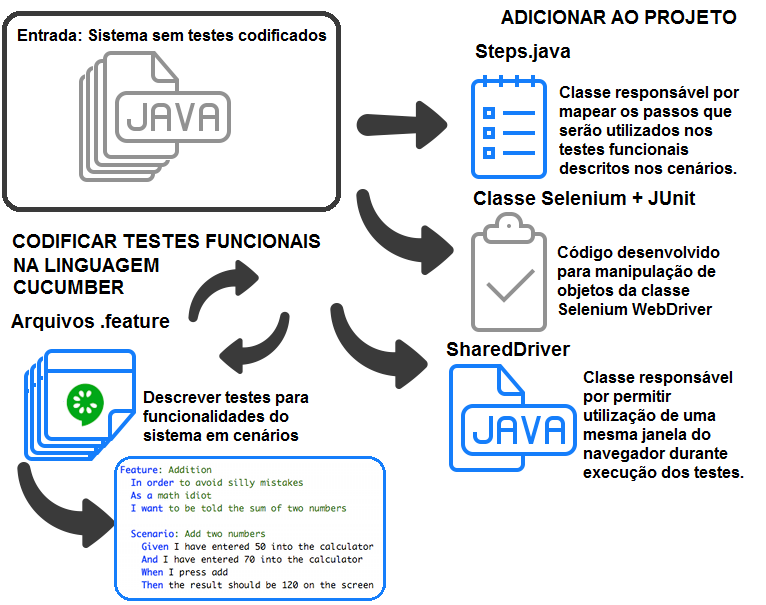
\includegraphics[width=0.8\textwidth]{solucao2}
	\caption{Estrutura da solução utilizando Selenium e Cucumber.}
	\label{fig:solucao2}
\end{figure}

A solução é composta por três estágios, onde no primeiro será inserido no projeto a classe genérica de testes já descrita, porem dela só serão utilizados os métodos que descrevem ações do Selenium WebDriver. No segundo estágio ocorre a adição de uma classe, onde são apresentados métodos que representam \emph{steps} da linguagem Cucumber o que possibilita descrever, no ultimo estágio, cenários no Cucumber em arquivos \texttt{.feature}, que descrevem casos de teste para as funcionalidades codificadas no sistema. A imagem \ref{fig:solucao2} apresenta esse fluxo.

\subsection{Classe genérica de testes}
Na classe genérica de testes foram mantidos os métodos anteriormente utilizados que permitiam gerenciar ações do Selenium WebDriver, como apresenta a figura \ref{code:Classe genérica contendo métodos WebDriver}.
Entretanto, foram removidos os métodos que realizavam os testes com base nas anotações inseridas nas classes Java do projeto.

\begin{figure}[!htt]
	\begin{lstlisting}
public Object getValorPropriedadeCampo(WebElement webElement, String atributo) {
    if (atributo.equals(ATRIBUTO_COMPARACAO_ASSERT_TEXTO)) {
        return webElement.getText();
    } else if (atributo.equals(ATRIBUTO_COMPARACAO_ASSERT_NOME_TAG)) {
        return webElement.getTagName();
    } else if ...
} //Retorna atributo de um campo

//Retorna um elemento HTML
public WebElement getEncontraCampo(String identificador, String campo) { 
    return webDriver.findElement(getEncontra(identificador, campo));
}

public By getEncontra(String identificador, String campo) {
    if (identificador.equals(IDENTIFICADOR_ID)) {
        return By.id(campo);
    } else if (identificador.equals(IDENTIFICADOR_NOME)) {
        return By.name(campo);
    } else if ...
}
	\end{lstlisting}
	\caption{Métodos para busca de elemento web utilizando Selenium WebDriver}
	\label{code:Classe genérica contendo métodos WebDriver}
\end{figure}

\subsection{Classe que descreve \emph{steps}}
A classe \texttt{Steps.java} foi criada com intuito de realizar o elo de ligação entre as ações da classe WebDriver e frases utilizadas nos arquivos \texttt{.feature} da linguagem Cucumber. Nesta classe foram confeccionados métodos que mapeiam ações do Cucumber e, dentro dos mesmos, ocorrem as chamadas dos métodos da classe WebDriver como ilustra o código em \ref{code:Classe com Steps Cucumber}.

\begin{figure}[!htt]
	\begin{lstlisting}
    @Dado("^atribuir timeout navegador (\\d+)$")
    public void setTimeoutNavegador(int timeout) {
        webDriver.manage().timeouts().implicitlyWait(timeout, TimeUnit.SECONDS);
    }

    @Dado("^acesso o endereco (.*)$")
    public void acessarEndereco(String url) {
        webDriver.get(TestePropriedades.urlSistema + url);
    }

    @Quando("^seleciono a opcao (.*) no campo (.*) buscando pelo (.*)$")
    public void selecionarOpcaoCampo(String opcao, String campo, String identificador) {
        WebElement webElement = getEncontraCampo(identificador, campo);
        if (webElement != null) {
            Select select = new Select(webElement);
            select.selectByVisibleText(opcao);
        }
    }

    @E("^limpo o campo (.*) buscando pelo (.*)$")
    public void limparCampo(String campo, String identificador) {
        WebElement webElement = getEncontraCampo(identificador, campo);
        if (webElement != null) {
            webElement.clear();
        }
    }

    @E("^preencho o campo (.*) com o valor (.*) buscando pelo (.*)$")
    public void preencherCampo(String campo, String valor, String identificador) {
        WebElement webElement = getEncontraCampo(identificador, campo);
        if (webElement != null) {
            webElement.sendKeys(valor);
        }
    }

    @E("^clico no elemento (.*) buscando pelo (.*)$")
    public void clicarElemento(String campo, String identificador) {
        WebElement webElement = getEncontraCampo(identificador, campo);
        if (webElement != null) {
            webElement.click();
        }
    }
    
    @E("^submeto o elemento (.*) buscado pelo (.*)$")
    public WebElement submeterElemento(String campo, String identificador) {
        WebElement webElement = funcoes.getEncontraCampo(identificador, campo);
        if (webElement != null) {
            webElement.submit();
        }
        return webElement;
    }
	\end{lstlisting}
	\caption{Classe genérica contendo steps Cucumber que descrevem ações do Selenium WebDriver}
	\label{code:Classe com Steps Cucumber}
\end{figure}

A linguagem Cucumber, quando trabalha conjuntamente com Java, disponibiliza anotações como: \texttt{@Dado, @Quando, @E e @Entao}, que corresponde de forma 1 para 1 frases descritas nos arquivos \texttt{.feature}.
Como podemos ver na ilustração, cada método que corresponde a um \emph{Step} do Cucumber apresenta uma anotação que identifica o mesmo, contendo uma frase fixa e parâmetros que são esperados. Dessa forma, podem-se descrever frases que correspondam a pequenas ações executadas em um navegador. Assim, cada método é responsável por executar uma ação específica, tornando possível reutilizar estes métodos para compor os cenários que posteriormente serão descritos.

Para tornar a solução mais completa, inseriu-se nessa classe, métodos que permitissem manipular campos que dependessem de chamadas Ajax e JavaScript, como demonstra a imagem \ref{code:Método WebDriverWait}

\begin{figure}[!htt]
	\begin{lstlisting}
@E("^aguardo (\\d+) milisegundos para verificar se elemento (.*) buscando pelo (.*) esta presente$")
public void aguardarCampoExistente(Long tempo, String campo, String identificador) {
    WebDriverWait webDriverWait = new WebDriverWait(webDriver, tempo);
    webDriverWait.until(ExpectedConditions.presenceOfElementLocated(
        funcoes.getEncontra(identificador, campo)));
}

@E("^aguardo (\\d+) milisegundos para verificar se elemento (.*) buscando pelo (.*) esta visivel$")
public void aguardarCampoVisivel(Long tempo, String campo, String identificador) {
    WebDriverWait webDriverWait = new WebDriverWait(webDriver, tempo);
    webDriverWait.until(ExpectedConditions.visibilityOf(funcoes.getEncontraCampo(identificador, campo)));
}

@E("^aguardo (\\d+) milisegundos para verificar se elemento (.*) buscando pelo (.*) desapareceu$")
public void aguardarCampoDesaparecer(Long tempo, String campo, String identificador) {
    WebDriverWait webDriverWait = new WebDriverWait(webDriver, tempo);
    webDriverWait.until(ExpectedConditions.invisibilityOfElementLocated(
        funcoes.getEncontra(identificador, campo)));
}
	\end{lstlisting}
	\caption{Método que permite manipulações com espera de tempo ou ação}
	\label{code:Método WebDriverWait}
\end{figure}

Essas ações são possíveis através da utilização dos métodos oferecidos pela classe \texttt{WebDriverWait} do Selenium.

\subsection{Descrição de cenários}
Após a inserção das duas classes Java apresentados anteriormente no projeto, torna-se possível escrever cenários que representem as funcionalidades que devem ser testadas.
Desta forma, pode-se criar arquivos \texttt{.feature} em que os cenários são compostos por uma sequência definida utilizando os passos descritos na classe \texttt{Steps}, onde a mesma realiza as ações em um navegador.
Podemos ver um exemplo desta abordagem no código apresentado em \ref{code:feature}.

\begin{figure}[!htt]
	\begin{lstlisting}
#language: pt

Funcionalidade: Ações executadas por um aluno do curso de Ciência da Computação no registro de seu
  plano individual de estudos complementares.

  Contexto: Fazer login no sistema como um aluno
    Dado acesso o endereco "/login.htm"
    Quando preencho o campo "login" com o valor "lamaral" buscando pelo "id"
    E preencho o campo "senha" com o valor "teste123" buscando pelo "id"
    E clico no elemento "button.btn.btn-default" buscando pelo "css"
    Entao verifico se atributo "nome tag" do elemento "id" buscando pelo "nome" não está nulo

  @aceitacao
  Cenario: Adicionar umas disciplina ao plano com sucesso.
    Dado seleciono a opcao "ELC1051 - Computação Gráfica Avançada (60h)" no campo "idDisciplinaAdicionar" buscando pelo "id"
    Quando preencho o campo "piecDisciplinaAdicionar.cursoOfertante" com o valor "Ciência da Computação" buscando pelo "id"
    E preencho o campo "piecDisciplinaAdicionar.semestreAnoRealizacao" com o valor "II/2011" buscando pelo "id"
    E clico no elemento "adicionarPiecDisciplina" buscando pelo "id"
    Entao comparo a igualdade entre o valor esperado "Sucesso!" com atributo "texto" do elemento "h4" buscando pelo "css"

  @rejeicao
  Cenario: Não permitir adicionar disciplina ao plano quando a mesma já está incluida.
    Dado seleciono a opcao "ELC1051 - Computação Gráfica Avançada (60h)" no campo "idDisciplinaAdicionar" buscando pelo "id"
    Quando preencho o campo "piecDisciplinaAdicionar.cursoOfertante" com o valor "Ciência da Computação" buscando pelo "id"
    E preencho o campo "piecDisciplinaAdicionar.semestreAnoRealizacao" com o valor "II/2011" buscando pelo "id"
    E clico no elemento "adicionarPiecDisciplina" buscando pelo "id"
    Entao comparo a igualdade entre o valor esperado "Disciplina já inserida no plano." com atributo "texto" do elemento "piec.errors" buscando pelo "id"
	\end{lstlisting}
	\caption{Testes de uma funcionalidade descrita por seus cenários em um arquivo .feature}
	\label{code:feature}
\end{figure}

Como visto em \ref{code:feature}, basta utilizar os passos previamente definidos nos métodos da classe \texttt{Steps.java} complementando apenas com os parâmetros necessários para identificação do elemento que se deseja manipular em uma tela do sistema web.

\subsection{Utilizando a mesma janela do navegador para execução dos testes}
Ao iniciar os testes na solução, após finalizar a codificação da mesma, notou-se que existia uma perda de tempo quando os testes eram executados, pois, a cada cenário executado o Selenium WebDriver fechava a janela do navegador ativa e, quando um novo cenário fosse executado, uma nova janela era aberta. Para evitar que este retrabalho fosse realizado e, assim, fosse possível reutilizar a janela do navegador ativa, encontrou-se na documentação existente na página da linguagem Cucumber\footnote{https://cucumber.io/} a solução para esta questão, utilizando a classe \texttt{SharedDriver} desenvolvida por Aslak Hellesoy e disponibilizada no projeto \texttt{cucumber-jvm\footnote{https://github.com/cucumber/cucumber-jvm/blob/master/examples/java-webbit-websockets-selenium/src/test/java/cucumber/examples/java/websockets/SharedDriver.java}}, onde deve-se instanciar um objeto desta classe no lugar da classe WebDriver, utilizada anteriormente.

\subsection{Validando solução em sistemas web}
Após a finalização da codificação da solução, iniciou-se a fase de validação e aplicação da solução utilizando Cucumber e Selenium em softwares web. Nesta etapa foram escolhidos dois softwares web, que respeitassem os requisitos existentes no escopo delimitado pelo projeto em questão. 

O primeiro sistema escolhido foi um sistema desenvolvido para efetuar a solicitação de disciplinas complementares de graduação, do curso de Ciência da Computação, da Universidade Federal de Santa Maria. Sistema esse que pode ser definido como de pequeno porte, pois possui poucas telas e processo bem definido, utilizando apenas recursos como: Ajax, Javascript e JasperReport, para geração de relatórios.

O Segundo sistema, em que os testes funcionais seriam aplicados, seria um software de uma empresa privada, da região de Santa Maria, chamada Megatecnologia. Este software comercializado como SILAS BPMs, apresenta
um sistema voltado para modelagem de processo BPMs, no qual é possível descrever etapas, tramitações, telas e campos de um processo. Este sistema apresenta complicações bem maiores que o primeiro, por tratar-se de um sistema comercializado há mais de 8 anos, onde existe a utilização de tecnologias como: Ajax, geração de documentos em XLS e PDF, comunicação via WebService, geração de gráficos e mapas, utilizando API`s do Google e, além disso, possuir um processo que é descrito pelo usuário, tornando mais difícil escrever um teste funcional, em que se sabe com certeza o estado atual de um campo.

\subsubsection{Aplicando solução no sistema de registro de disciplinas Complementares}
Para realização desta tarefa, foram utilizadas as funcionalidades descritas no documento de especificação deste software para validar se o mesmo apresenta todas as funcionalidades que se compromete a atender.
Como o processo apresenta dois atores principais, onde o primeiro seria o aluno e, o segundo, um membro do colegiado do curso, foram separados os testes em dois arquivos \texttt{.feature}. O primeiro contendo ações realizadas por alunos e, o segundo, para ações que um membro do colegiado executa.

Como forma de reduzir o trabalho de um desenvolvedor de teste, utilizando os recursos disponibilizados pela linguagem Cucumber, pode-se utilizar o recurso \texttt{Contexto} para descrever uma sequência de passos que deverá ser executada para cada um dos cenários de uma funcionalidade. Assim, evita-se de ter que reescrever a mesma sequência de passos para todos os cenários. A imagem \ref{code:Contexto} exemplifica essa utilização.

\begin{figure}[!htt]
	\begin{lstlisting}
Funcionalidade: Ações executadas por um membro do colegiado do curso de Ciência da Computação na aprovação/regeição de planos individuais de estudos complementares.

  Contexto: Fazer login no sistema como um membro do colegiado
    Dado acesso o endereco "/login.htm"
    Quando preencho o campo "login" com o valor "colegiado" buscando pelo "id"
    E preencho o campo "senha" com o valor "colegiado123" buscando pelo "id"
    E clico no elemento "button.btn.btn-default" buscando pelo "css"
    Entao verifico se atributo "nome tag" do elemento "id" buscando pelo "nome" não está nulo
	\end{lstlisting}
	\caption{Exemplo de utilização do Contexto em um arquivo Cucumber}
	\label{code:Contexto}
\end{figure}

O \texttt{Contexto} deve ser descrito no inicio do código de uma funcionalidade, antes dos cenários do mesmo.

Outro recurso da linguagem Cucumber útil para redução na escrita de novos testes, é a \texttt{Delineacao do Cenario}, que permite reutilizar o mesmo cenário, aplicando os
valores contidos em uma tabela descrita pelo recurso \texttt{Exemplos} como mostra o código \ref{code:Delineacao}

\begin{figure}[!htt]
	\begin{lstlisting}
Delineacao do Cenario: 1 - Não permitir inserir no PIEC disciplina que não faça parte do curso, sem o preenchimento do campo relevância da integralização
     2 - Não permitir cadastrar nova instituição com sigla já cadastrada
     3 - Não permitir cadastrar nova disciplina sem sua respectiva sigla
     4 - Não permitir cadastrar nova disciplina sem sua respectiva nome
     5 - Não permitir inserir disciplina com uma sigla já cadastrada
    Dado seleciono a opcao "Adicionar outra disciplina" no campo "idDisciplinaAdicionar" buscando pelo "id"
    Quando preencho o campo "novaDisciplina.codigo" com o valor <codigoDis> buscando pelo "id"
    E preencho o campo "novaDisciplina.nome" com o valor <nomeNovaDisciplina> buscando pelo "id"
    E preencho o campo "piecDisciplinaAdicionar.relevanciaIntegralizacao" com o valor <relevancia> buscando pelo "id"
    E seleciono a opcao "Adicionar outra instituição" no campo "novaDisciplina.idInstituicao" buscando pelo "id"
    E seleciono a opcao "78 horas" no campo "novaDisciplina.cargaHoraria" buscando pelo "id"
    E preencho o campo "novaInstituicao.nome" com o valor "Universidade Teste" buscando pelo "id"
    E preencho o campo "novaInstituicao.sigla" com o valor <siglaInst> buscando pelo "id"
    E preencho o campo "piecDisciplinaAdicionar.arquivoPlanoEnsino" com o valor "C:\\arquivo.pdf" buscando pelo "id"
    E clico no elemento "adicionarPiecDisciplina" buscando pelo "id"
    Entao comparo a igualdade entre o valor esperado <msgErro> com atributo "texto" do elemento "piec.errors" buscando pelo "id"

  Exemplos:
    | codigoDis | nomeNovaDisciplina | relevancia | siglaInst | msgErro                     |
    | TESTE95   | Teste informática  |            | USC       | Preencha o campo relevância.|
    | TESTE95   | Teste informática  | Teste 1    | UFSM      | Sigla já cadastrada         |
    |           | Teste informática  | Teste 2    | UFT       | Preencha o campo código.    |
    | TESTE98   |                    | Teste 3    | UFS       | Preencha o campo nome.      |
    | ELC1051   | Computação Gráfica | Teste 4    | UFAR      | Código já cadastrado.       |
	\end{lstlisting}
	\caption{Cenário executado para cada linha existente na tabela Exemplos}
	\label{code:Delineacao}
\end{figure}

Em \texttt{Delineacao do Cenario} ao invés de ser inseridos valores para testes, são informados os rótulos existentes no cabeçalho da tabela do recurso \texttt{Exemplos}. Desta forma, quando o teste for ser executado, esse valor será substituído, em tempo de execução, pelo valor existente nessa coluna para cada uma das linhas da tabela.

Utilizando-se destes recursos concluiu-se, de forma satisfatória, a codificação de cenários de testes para todos os requisitos existentes neste sistema.

\subsubsection{Aplicando solução no sistema SILAS BPMs}
Para o software em questão, por tratar-se de um sistema que possui mais de oito anos de desenvolvimento e por não possuir nenhum tipo de teste automatizado codificado, optou-se por retirar do \emph{task bord}, onde a equipe de desenvolvimento, da empresa em questão, gerenciava tarefas a desenvolver e desenvolvidas, as ultimas funcionalidades finalizadas para descreve-las como cenários e, assim, realizar os primeiros testes.
Logo no início do mapeamento dos testes, notaram-se necessidades que o sistema de registros de disciplinas complementares não possuía. Como, por exemplo, a necessidade de guardar valores de um campo para, após submeter alguma função, comparar com o novo valor do campo em questão. Também percebeu-se a indispensabilidade de permitir ações condicionais nos testes. Essa necessidade se deu pelo fato de, em alguns casos, não se conhecer o estado atual de algum elemento na tela em questão e, desta forma, o teste poderia falhar mesmo quando não existisse problema.
Após algumas tentativas de utilizar a solução proposta para esses novos cenários, notou-se que seria inviável trabalhar sem que essas questões fossem viabilizadas.

\subsection{Considerações sobre a solução Cucumber e Selenium}
Com o avanço na confecção de testes aplicados em sistemas reais, percebeu-se uma série de vantagens e desvantagens na utilização desta solução no processo de desenvolvimento e testes de funcionalidades.
Como vantagens, podemos elencar o fato de, ao escrever cenários utilizando o IDE que tenha suporte para a linguagem Cucumber, pouco se escreve, reutilizando sempre os \emph{steps} descritos na classe \texttt{Steps.java}. Sendo, assim, necessário apenas informar os parâmetros esperados pelos mesmos. Ainda destaca-se o fato de os cenários descreverem, de forma simples, o que deve ocorrer na funcionalidade testada e, desta forma, serve também como documentação.
Quando pensamos nos pontos fracos da solução, podemos destacar os empecilhos detectados no desenvolvimento de testes para a aplicação SILAS BPMs. Somam-se a estes, algumas limitações que a linguagem Cucumber possui, como o fato de não ser possível reutilizar um cenário dentro de outro cenário\footnote{Essa funcionalidade estava disponível na primeira versão da linguagem, mas a mesma foi removida. Embora o exemplo pode fazer sentido quando se trabalha de forma sequencial através dos cenários a longo prazo produz-se cenários que são difíceis de manter e entender \cite{givenscenario}. } ou até mesmo utilizar como parâmetro valores que diferem dos tipos comuns da linguagem Java (int, float, String). Outro fator problemático nessa solução é o fato de todos os dados utilizados nos testes serem persistidos e, com isso, ser necessário a restauração manual do ultimo estado válido da base de dados onde os testes se realizam.

\section{Solução para testes funcionais com Selenium WebDriver}
Como forma de possibilitar a utilização de testes condicionais, armazenamento de valores e manipulação de objetos Java dentro do testes funcionais, optou-se pela confecção de uma nova abordagem neste projeto, mesmo que para isso se tivesse que abdicar da praticidade e interface amigável do Cucumber. Assim, os testes funcionais seriam descritos diretamente em classes de teste Java. A imagem \ref{fig:solucao3} apresenta essa pequena alteração na abordagem dos testes proposta. 

\begin{figure}[!htb]
	\centering
	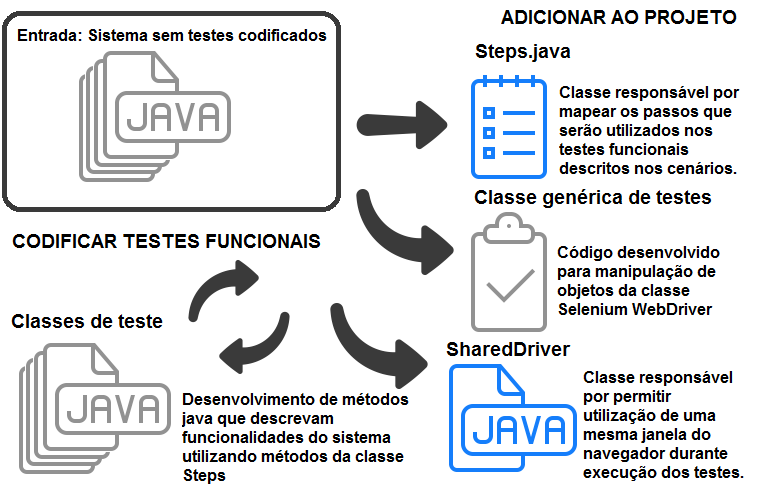
\includegraphics[width=0.8\textwidth]{solucao3}
	\caption{Estrutura da solução utilizando somente Selenium.}
	\label{fig:solucao3}
\end{figure}

\subsection{Classes Java contendo testes funcionais}
Como descrito na imagem \ref{fig:solucao3}, esta abordagem reutiliza praticamente toda a estrutura existente na abordagem Cucumber e Selenium, com isso, somente os arquivos onde são escritos os cenários mudam. Ao invés de criarmos arquivos \texttt{.feature}, contento as funcionalidades e cenários que serão testados, tem-se, agora, classes Java de teste, que são responsáveis por descrever os testes.
Na figura \ref{code:seleniumTeste} temos um exemplo de um cenário descrito utilizando a abordagem atual.  Pode-se notar que os métodos da classe \texttt{Steps.java} ainda são utilizados, porém de forma direta.

\begin{figure}[!htt]
	\begin{lstlisting}
	
	/*
		Quando um agrupamento é fechado, o sistema deve alterar a data de fechamento do mesmo para a data atual. No caso da caixa atual estar aberta
	*/
	private void abreFechaAgrupamento() {
		navegador.clicarElemento("img[alt=\"Visualizar\"]", Steps.IDENTIFICADOR_CSS);
		navegador.aguardarCampoVisivel(100l, "img[alt=\"F\"]", Steps.IDENTIFICADOR_CSS);
		WebElement dataAbertura = navegador.getEncontraCampo("data_abertura_agrupamento_1");
		WebElement dataFechamento = navegador.getEncontraCampo("data_fechamento_agrupamento_1");
		boolean aberto = true;
		if (dataAbertura.getText() != null) {
			aberto = false;
		}
		navegador.clicarElemento("img[alt=\"F\"]");
		if (aberto) {
			assertEquals(SilasFuncoesDatas.sdf.format(new Date()), dataFechamento.getText());
		} else {
			assertEquals(SilasFuncoesDatas.sdf.format(new Date()), dataAbertura.getText());
		}
	}	
	\end{lstlisting}
	\caption{Teste funcional utilizando abordagem Selenium WebDriver}
	\label{code:seleniumTeste}
\end{figure}

Por tratar-se de código Java, além de tornar possível utilizar testes condicionais e armazenamento de valores, novas funções tornaram-se plausíveis, como apresentado no código \ref{code:seleniumDate}, onde realiza-se comparações com uma data utilizando um formato específico.

\begin{figure}[!htt]
	\begin{lstlisting}

	/*
		Quando navagamos pelos agrupamentos, verificamos que as datas de abertura das caixas não são necessariamente as mesmas.
	*/		
	private void navegarEntreAgrupamentos() {
		navegador.clicarElemento("imagem_anterior_agrupamento_1");
		assertNotEquals(SilasFuncoesDatas.sdf.format(new Date()), navegador.getEncontraCampo("data_abertura_agrupamento_1").getText());
	}
	
	\end{lstlisting}
	\caption{Realizando comparações utilizando o tipo de dados data.}
	\label{code:seleniumDate}
\end{figure}

Pode-se, também, localizar valores que não são estáticos na busca de elementos HTML existentes na tela atual de manipulação, como demonstra o trecho de código \ref{code:seleniumBuscaId}.

\begin{figure}[!htt]
	\begin{lstlisting}
	@Test
	//Colocar datas ao lado da indentificação do agrupamento (bateria), para assim contemplar as necessidades da embrapa acre
	public void datasInicioFimBateria() {
		navegador.acessarEndereco(url + "/gerenciar-agrupamentos.htm");
		String idAgrupamento = navegador.getEncontraCampo(Steps.IDENTIFICADOR_ID, "id").getText();
		Agrupamento agrupamento = service.getAgrupamento(Long.valueOf(idAgrupamento));
		navegador.getEncontraCampo("data_abertura_agrupamento_" + agrupamento.getId());
		navegarEntreAgrupamentos();
	}	
	\end{lstlisting}
	\caption{Realizando comparações utilizando o tipo de dados data.}
	\label{code:seleniumBuscaId}
\end{figure}


\subsection{Validando solução em sistemas web}
Para validar esta solução, foram utilizados os mesmos dois projetos já usados na solução anterior.

\subsubsection{Aplicando solução no sistema de registro de disciplinas Complementares}
Como ocorrido com a solução anterior, essa solução viabiliza a codificação de testes para todos os requisitos funcionais deste software. Ilustração \ref{code:seleniumPiec} trás a codificação do mesmo teste executado na imagem \ref{code:Contexto}.

\begin{figure}[!htt]
	\begin{lstlisting}
@Test
/*Fazer login no sistema como um membro do colegiado*/
public void getLoginMembroColegiado() {
    steps.acessarEndereco("/login.htm");
    steps.preencherCampo("login", "colegiado", TesteFormulario.IDENTIFICADOR_ID);
    steps.preencherCampo("senha", "colegiado123", TesteFormulario.IDENTIFICADOR_ID);
    steps.clicarElemento("button.btn-default", TesteFormulario.IDENTIFICADOR_CSS);
    steps.compararSeNaoNulo(TesteFormulario.ATRIBUTO_COMPARACAO_ASSERT_NOME_TAG, "id", TesteFormulario.IDENTIFICADOR_NOME);
}
	\end{lstlisting}
	\caption{Cenário descrevendo mesma funcionalidade contida em \ref{code:Contexto}}
	\label{code:seleniumPiec}
\end{figure}

\subsubsection{Aplicando solução no sistema SILAS BPMs}
Ao contrário do ocorrido com a aplicação de registro de disciplinas complementares do curso de Ciência da Computação da Universidade Federal de Santa Maria (UFSM), a solução que mescla a utilização da linguagem Cucumber juntamente com o \emph{framework} Selenium WebDriver não contemplava, na totalidade, os testes necessários. Agora utilizando essa nova abordagem, tornou-se viável a codificação dos testes necessários e, com isso, optou-se, na empresa Megatecnologia, pela continuidade da realização de testes através desta solução.

\subsection{Considerações sobre a solução Selenium WebDriver}
A abordagem em questão, assim como as anteriores, apresenta vantagens e desvantagens. Como vantagem, pode-se elencar o fato de, por trabalhar somente com a linguagem Java, possibilitar uma série de ações, que não seriam possíveis, utilizando Cucumber na composição da solução. Como por exemplo, a utilização de testes condicionais, laços de repetição, busca de valores de um objeto Java, assim como manipulação de tipos que não façam parte dos tipos nativos da linguagem Java. Apesar disso, a solução apresenta um cenário mais complexo de ser entendido por qualquer interessado do projeto, comparado a solução utilizando Cucumber. Apresenta também, descrições mais poluídas visualmente e mais distantes de uma linguagem natural, além de possuir o mesmo problema referente à restauração da base de dados, após execução dos testes.

\chapter{Resultados}
Como forma de validação das abordagens criadas neste trabalho, onde as mesmas visam a redução do trabalho para uma equipe de teste e desenvolvimento, realizou-se comparações que serviriam para levantar o ganho em utilizar uma abordagem ou outra. 

\section{Comparando abordagens funcionais}
Mesmo conhecendo as principais virtudes das abordagens criadas e, também em quais escopos as mesmas funcionavam de forma adequada, ainda era necessário expor o ganho em utilizar umas dessas abordagens ao invés de criar um teste funcional somente utilizando métodos que as ferramentas de teste web disponibilizam.

Como forma de medir este ganho, resolveu-se descrever uma funcionalidade do sistema de registro de disciplina complementares, utilizando tanto a abordagem Cucumber e WebDriver, como a abordagem WebDriver e, por fim, criando um teste utilizando apenas os métodos disponíveis da ferramenta Selenium. Essas diferenças são apresentadas nas imagens \ref{code:seleniumAddDisciplina}, \ref{code:solucao2AddDisciplina} e \ref{code:solucao3AddDisciplina}.


\begin{figure}[!htt]
	\begin{lstlisting}
Cenario: Cadastrar nova disciplina.
    Dado acesso o endereco "/cadastro-disciplina.htm"
    Quando preencho o campo "codigo" com o valor "ELC9898" buscando pelo "id"
    E preencho o campo "nome" com o valor "Disciplina nova" buscando pelo "id"
    E seleciono a opcao "60" no campo "cargaHoraria" buscando pelo "id"
    E clico no elemento "ativa1" buscando pelo "id"
    E seleciono a opcao "UFSM - Universidade Federal de SM" no campo "idInstituicao" buscando pelo "id"
    E clico no elemento "preAprovada1" buscando pelo "id"
    E clico no elemento "salvar" buscando pelo "id"
    Entao comparo a igualdade entre o valor esperado "Sucesso!" com atributo "texto" do elemento "h4" buscando pelo "css"
	\end{lstlisting}
	\caption{Teste utilizando solução Cucumber e WebDriver}
	\label{code:solucao2AddDisciplina}
\end{figure}

\begin{figure}[!htt]
	\begin{lstlisting}
//Cadastrar nova disciplina
public void cadastrarDisciplina() {
    steps.acessarEndereco("/cadastro-disciplina.htm");
    steps.preencherCampo("codigo", "ELC9898", TesteFormulario.IDENTIFICADOR_ID);
    steps.preencherCampo("nome", "Disciplina nova", TesteFormulario.IDENTIFICADOR_ID);
    steps.selecionarOpcaoCampo("60", "cargaHoraria", TesteFormulario.IDENTIFICADOR_ID);
    steps.clicarElemento("ativa1");
    steps.selecionarOpcaoCampo("UFSM - Universidade Federal de SM", "idInstituicao", "id");
    steps.clicarElemento("preAprovada1");
    steps.clicarElemento("salvar");
    steps.compararIgualdade("Sucesso!", "texto", "h4", "css");
}
	\end{lstlisting}
	\caption{Teste utilizando solução WebDriver}
	\label{code:solucao3AddDisciplina}
\end{figure}

\begin{figure}[!htt]
	\begin{lstlisting}
	@Test
	public void cadastrarDisciplinaSucesso() {
	WebDriver webDriver = new FirefoxDriver();
	webDriver.get(url + "/cadastro-disciplina.htm");
	webDriver.findElement(By.id("codigo")).sendKeys("ELC9898");
	webDriver.findElement(By.id("nome")).sendKeys("Disciplina nova");
	Select cargaHoraria = new Select(webDriver.findElement(By.id("cargaHoraria")));
	cargaHoraria.selectByVisibleText("60");
	webDriver.findElement(By.id("ativa1")).click();
	Select instituicao = new Select(webDriver.findElement(By.id("idInstituicao")));
	instituicao.selectByVisibleText("UFSM - Universidade Federal de SM");
	webDriver.findElement(By.id("preAprovada1")).click();
	webDriver.findElement(By.id("salvar")).click();
	assertEquals("Sucesso!", webDriver.findElement(By.cssSelector("h4")).getText());
	}
	\end{lstlisting}
	\caption{Teste utilizando apenas o Selenium}
	\label{code:seleniumAddDisciplina}
\end{figure}

Como pode-se notar pelo código \ref{code:seleniumAddDisciplina}, \ref{code:solucao2AddDisciplina} e \ref{code:solucao3AddDisciplina}, existe uma diminuição no número de linhas
escritas nos testes que exploram as duas abordagens deste trabalho em relação a codificação utilizando apenas o \emph{framework} Selenium. Durante a realização dessas
comparações percebeu-se, também, uma possível redução de caracteres digitados utilizando as abordagens apresentadas, isso quando trabalha-se com um IDE que possua suporte
para as linguagens em questão. Por fim, pode-se também levantar suspeita que a abordagem Cucumber e WebDriver trás ganhos na leitura dos testes, que se tornam mais
compreensíveis, mesmo que não se entenda de linguagens de programação.

\section{Comparando as três soluções propostas}
Visando mapear, de forma mais externa, as abordagens desenvolvidas, confrontou-se as soluções propostas elencando suas respectivas virtudes e limitações e, com isso, torna-se possível realizar escolhas sobre qual abordagem é mais apropriada para um cenário específico que se apresente.
Por exemplo, quando a equipe decide que serão necessários apenas a realização de testes unitários, a abordagem para testes unitários que utiliza anotações apresenta-se como uma boa alternativa, pois a mesma possui recursos que permitem realizar este tipo de teste e, ao mesmo tempo, não necessita de codificação em classes de teste, pois a simples inserção de anotações nas classes do modelo é suficiente.

Quando deseja-se realizar testes funcionais e não se faz necessário utilizar verificações condicionais, adotar a segunda solução torna-se uma opção válida. A utilização do Cucumber, neste casos, torna-se prática e ainda possibilita que qualquer \emph{stakeholder} do projeto entenda as funcionalidades descritas pelos testes.
A ultima abordagem pode ser apropriada, quando o sistema em questão é mais complexo e necessita de maiores validações.

A tabela \ref{tab:comparacaoSolucoes} apresenta os principais pontos fortes e as maiores fraquezas dessas três abordagens.

\begin{table}[!htpb]
	\centering
	\begin{tabular}{p{5cm}|c|c|c}
		& Unitário & Cucumber e Selenium & Funcional Selenium\\ \hline
		Testes unitários & \checkmark & \checkmark & \checkmark \\ \hline
		Testes funcionais &  & \checkmark & \checkmark \\ \hline
		Elementos que dependam de funções Ajax e Javascript & & \checkmark & \checkmark \\ \hline
		Cenários com escrita de fácil compreensão & & \checkmark & \\ \hline
		Realização de testes dependentes de condições & & & \checkmark \\ \hline
		Armazenar valor de um campo para utiliza-lo posteriormente & & & \checkmark \\ \hline
		Possibilita utilizar parâmetros que diferem dos tipos básicos (int, float, String) & \checkmark & & \checkmark \\ \hline
		Retroceder o banco de dados ao último estado válido após realizar os testes & & & \\ \hline
		Utilização de cenários dentro de outro cenário & & & \checkmark \\ \hline
	\end{tabular}
	\caption{Vantagens e desvantagens das abordagens de teste confeccionadas}
	\label{tab:comparacaoSolucoes}
\end{table}

\chapter{Conclusão}
A proposta inicial deste trabalho consistia em apresentar uma solução em forma de códigos de teste, que permitisse o reaproveitamento e reutilização dos mesmo, acarretando em um menor esforço na codificação de novos testes para sistemas web, desenvolvidos em Java. Entretanto, o resultado final, obtido pelo trabalho em questão, trata-se não de uma solução, mas, sim, de três abordagens utilizando ferramentes para teste de software que diferem entre si, cada uma possuindo ponto fortes e pontos fracos e sendo mais relevante para uma determinada situação. A condução e criação dessas abordagens foram tomadas, ao longo do desenvolvimento, a partir dos percalços e necessidades que apareciam e em meio a validação das abordagens em questão.

Como contribuição, este trabalho apresenta uma abordagem que mescla a utilização da linguagem Cucumber com o \emph{framework} Selenium Webdriver, apresentando passos, que podem tornar o processo de criação dos testes em uma tarefa mais prática e rápida, sendo, assim, necessário apenas descrever cenários que correspondem a funcionalidades do sistema.

A lista a seguir expõe, em ordem de relevância, algumas melhorias que poderiam ser incorporadas em uma nova versão deste projeto:

\begin{itemize}
	\item Apresentar no auto completar do IDE, os campos pertencentes ao contexto atual do .feature: Ao utilizar um IDE que possibilite manipulação de plugins, desenvolver mecanismo que pesquise nos arquivos JSP/JSF todos os campos referentes à um contexto atual, e assim apresente sugestão de autocompletar para os cenários que estão sendo descritos pelo Cucumber.
	\item Não persistir no BD as alterações realizadas pelos testes automatizados: Possibilitar que ao finalizar execução de um teste funcional, o bando de dados utilizado retorne ao estado inicial, não persistindo assim as alterações realizadas pelos testes executados.
	\item Criar mecanismo que busque na árvore do projeto classes de validação dos formulários e transcreva essas informações em cenários de teste Cucumber: Criar mecanismo que permita gerar testes a partir das validações que são inseridas nas classes de validação referentes a uma classe de controle.
\end{itemize}

\setlength{\baselineskip}{\baselineskip}
\bibliographystyle{abnt}
\bibliography{../referências}
\end{document}